%%%%%%%%%%%%%%%%%%%%%%% file template.tex %%%%%%%%%%%%%%%%%%%%%%%%%
%
% This is a general template file for the LaTeX package SVJour3
% for Springer journals.          Springer Heidelberg 2010/09/16
%
% Copy it to a new file with a new name and use it as the basis
% for your article. Delete % signs as needed.
%
% This template includes a few options for different layouts and
% content for various journals. Please consult a previous issue of
% your journal as needed.
%
%%%%%%%%%%%%%%%%%%%%%%%%%%%%%%%%%%%%%%%%%%%%%%%%%%%%%%%%%%%%%%%%%%%
%
% First comes an example EPS file -- just ignore it and
% proceed on the \documentclass line
% your LaTeX will extract the file if required
%
\RequirePackage{fix-cm}
\documentclass{svjour3}                     % onecolumn (standard format)
%\documentclass[smallcondensed]{svjour3}     % onecolumn (ditto)
%\documentclass[smallextended]{svjour3}       % onecolumn (second format)
%\documentclass[twocolumn]{svjour3}          % twocolumn
\smartqed  % flush right qed marks, e.g. at end of proof
\usepackage{graphicx}
%\usepackage{url}
\usepackage[hyphens]{url}
\usepackage{hyperref}
%\usepackage{mathptmx}      % use Times fonts if available on your TeX system
%\usepackage{latexsym}
%\newcommand{}{}
%Insert the name of "your journal" with
\journalname{Environmental Earth Sciences}
\hyphenation{ap-proa-ches}
%==================================================================================================
\begin{document}
\title{GeomInt}
\subtitle{Geomechanical integrity of host and barrier rocks - experiment, modeling and analysis of discontinuities}
%\titlerunning{Short form of title}        % if too long for running head
\author{Olaf Kolditz \and co-authors}
%\authorrunning{Short form of author list} % if too long for running head
\institute{B. Kolditz (corresponding author) \at
              %JLab, D-04318 Leipzig, Permoserstr. 15  \\
              %Tel.: +49-341-235-1031\\
              \email{ees-editor@web.de}           %  \\
%             \emph{Present address:} of F. Author  %  if needed
}
\date{Version: \today / Received: date / Accepted: date}
%--------------------------------------------------------------------------------------------------
\maketitle
%--------------------------------------------------------------------------------------------------
\begin{abstract}
GeomInt ...

\keywords{GeomInt \and OpenGeoSys}
\end{abstract}
%--------------------------------------------------------------------------------------------------
\section{Introduction}
\label{sec:intro}

Introduction ...

\begin{figure}[ht!]
\centering
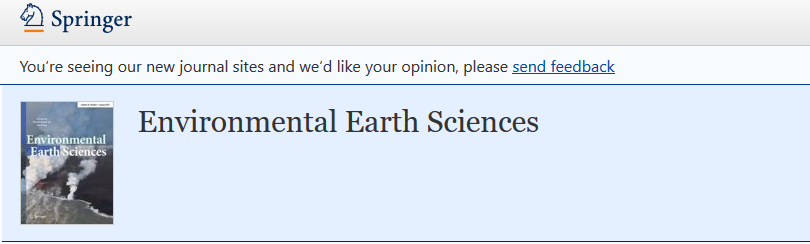
\includegraphics[width=1.00\columnwidth]{fig01a.png}
\caption{A glimpse of the new EES website: \url{https://www.springer.com/journal/12665}}
\label{fig:01}
\end{figure}

%--------------------------------------------------------------------------------------------------
\section{Methods}
\label{sec:methods}

Methods, citation \cite{Shirzadi2017a}

%--------------------------------------------------------------------------------------------------
\section{Results and Discussion}
\label{sec:results}

small changes

%--------------------------------------------------------------------------------------------------
\section{Conclusions}
\label{sec:conclusions}

%--------------------------------------------------------------------------------------------------
\begin{acknowledgements}
The funding of the GeomInt project by the Federal Ministry for Education and Research (BMBF) under grant 03G0866A is highly acknowledged.
\end{acknowledgements}
%--------------------------------------------------------------------------------------------------
% BibTeX users please use one of
%\bibliographystyle{spbasic}      % basic style, author-year citations
%\bibliographystyle{spmpsci}      % mathematics and physical sciences
%\bibliographystyle{spphys}       % APS-like style for physics
%\bibliographystyle{plainnat}
%\bibliographystyle{plain}
\bibliographystyle{unsrt}
%\bibliographystyle{apalike}
\bibliography{literature}   % name your BibTeX data base
%--------------------------------------------------------------------------------------------------
\end{document}
%==================================================================================================

